\chapter{Preprocessing}

Data preparation takes 60 to 80 percent of the whole analytical pipeline in a typical machine learning project. It's very important to get an overview about the data before starting to build up a model. This seems to be a lot of time and effort, but will save you a lot of time afterwards \cite{naman18}. In many machine learning projects preprocessing is the most important part. A solid data basis can increase the performance of the model. Furthermore, preprocessed data is much more comfortable to deal with than raw data.

\section{Data Sources}
\label{chap:data-source}

The NLP model relies on two distinctive data sources. In detail, there is a single \emph{Personal Storage Table (PST) \footnote{An open proprietary file format by Microsoft used to store copies of messages}} for the email mailboxes \emph{info@mobiliar.ch} and \emph{meinemobiliar@mobiliar.ch}. For a better understanding, the two data sources are called \emph{infomobi} and \emph{meinemobi}. \emph{infomobi} is the single point of contact for every Swiss Mobiliar related question or request, whereas \emph{meinemobi} is only used by the clients of the \emph{"Meine Mobiliar"} customer platform. The platform gives you an overview of your active policies or lets you report a claim.

Both data sets contain email messages in three different formats. The most commonly used kind is \emph{HTML}, followed by some \emph{Plain Text} and even fewer \emph{RTF} messages.

\begin{figure}[!ht]
    \centering
    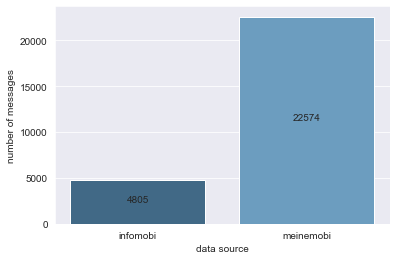
\includegraphics[scale=0.5]{plot-comparison-size}
    \caption{Size comparison of both data sources}
    \label{fig:plot-comparison-size}
\end{figure}

Figure \ref{fig:plot-comparison-size} shows, that the size of \emph{meinemobi} is more than four times larger than the size of \emph{infomobi}. Before pre-processing there is a total number of 27 379 messages. This is a solid base if we keep in mind, that a large part of the data may be removed at data cleansing. Afterwards, the remaining data needs to be labelled manually to build a model by supervised learning techniques.

\subsection{Comparison}

There are large differences between these two data sets. The distribution of message types hugely varies between them. As you can see in figure \ref{fig:plot-comparison-types}, about 80 percent of all messages are of type \emph{HTML}. This is consistent among the two different data sources. More interesting is the fact, that \emph{infomobi} contains more \emph{RTF} messages than \emph{Plain Text}, but very few of them are found in \emph{meinemobi}. This might be due to the large number of spam inside \emph{infomobi} which is often formatted as \emph{RTF}. One possible reason for the spam could be, that the generic email address of \emph{infomobi} is the victim of email harvesting\footnote{The discipline of obtaining email addresses through various methods like patterns}.

In addition to junk mails, \emph{infomobi} contains a lot more messages in foreign languages than \emph{meinemobi}. These messages must be removed, so the NLP model will only learn from German. A possible reason might be, that \emph{\textbf{info}@mobiliar.ch} is more international than the language specific \emph{meinemobi} address. Consider section \ref{chap:cleansing} to see how language detection is done.

\begin{figure}[!ht]
    \centering
    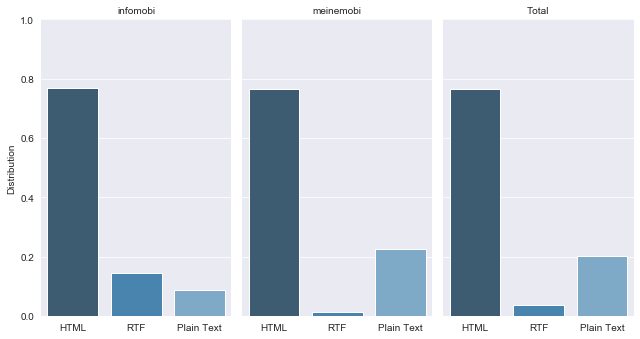
\includegraphics[scale=0.4]{plot-comparison-types}
    \caption{Distribution of the three message types}
    \label{fig:plot-comparison-types}
\end{figure}

Another important key figure is the typical length of a message. This key number can be measured in the total of words or characters. Figure \ref{fig:plot-comparison-words} shows that the statistical mean of words is 196.

The division of the number of characters by the amount of words provides an idea about the typical word in this specific context. Therefore the average word has a length of $8.45$ characters which is much higher than the average word in the \emph{Duden} corpus with its length of $6.09$ characters \cite{duden}. Possible reasons might be the formal language used in the business correspondence or insurance-related terms.

\begin{figure}[!ht]
    \begin{subfigure}{0.5\textwidth}
        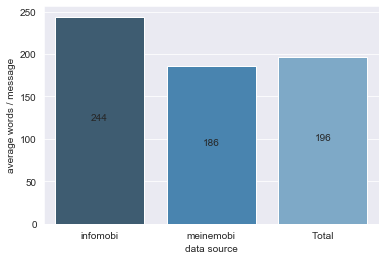
\includegraphics[scale=0.4]{plot-comparison-words}
        \caption{Comparison of words}
        \label{fig:plot-comparison-words}
    \end{subfigure}
    \begin{subfigure}{0.5\textwidth}
        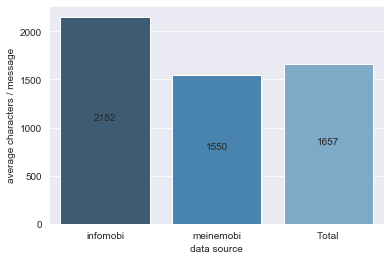
\includegraphics[scale=0.4]{plot-comparison-characters}
        \caption{Comparison of characters}
        \label{fig:plot-comparison-characters}
    \end{subfigure}
    \caption{Comparison of different indicators}
\end{figure}

\subsection{Typical Contents}
\label{chap:typical-contents}

Most messages can be divided into different groups. Such groups come very handy at the cleansing stage when patterns should be found to locate and remove junk from the remaining information. Therefore the \emph{mobi24} data can be splitted into several groups which are best described with sample messages.

\subsubsection{Spam and Junk}

Junk mails are much harder to detect today than they used to be in the past. Nowadays they are well written and mostly grammatically correct. Basically you could even use spam to train your model for certain use cases. But in that case spam should consistently be removed from the data set because it lacks of the insurance context which the model should get familiar with. The presence of links, the message length and the used language are often good indicators for detecting spam, especially when multiple indicators occur together.

\begin{quote}
    "Ein Ding der Unmöglichkeit! https://zixiseren1983.blogspot.in Auf Wiedersehen Elisabeth Speck"
\end{quote}

\begin{quote}
    "Mit der richtigen Haarpflege zur Traummähne :-) Die besten Pflegeprodukte für jeden Haartyp Endlich schöne Haare! Es ist Zeit, neue Haarprodukte zu entdecken..."
\end{quote}

\subsubsection{Auto-Generated Messages}

Some messages may not origin from real people but from machines instead. These group of messages is called \emph{automatically generated} and represents the largest group of messages an usual human receives per day. In the data source there are newsletters, notifications like payment success or delivery messages and failure reports present.

\begin{quote}
    "Fehler bei der Nachrichtenzustellung an folgende Empfänger oder Gruppen: generated1414@mobi.ch Die eingegebene E-Mail-Adresse konnte nicht gefunden werden..."
\end{quote}

\subsubsection{Customer Messages}

Moving forward, the messages which are actually written by humans and target Swiss Mobiliar's businesses are the only relevant ones for the model. There's a wide range of message types like sponsoring requests, claim notifications, and technical questions. All these messages share the same context.

Email messages are not as formal as letters and sometimes contain spelling errors. The texts are covered with typical Swiss expressions. There are even Swiss Mobiliar specific words like the name of products, magazines or applications. It's important to train the future model on this data to let it become aware of this typical kind of language.

\begin{quote}
    "Geschätzte Mobiliar ich habe mein Passwort verlegt. mit flotten Grüssen H. Muster"
\end{quote}

\begin{quote}
    "Guten Tag Im Anhang sende ich Ihnen die Offerte zum Schadenfall 8002.2533.9/XX zu. Wir bitten Sie die Offerte zu prüfen. Freundliche Grüsse Fritz Fischer"
\end{quote}

\section{Collecting Data}

As mentioned in \ref{chap:data-source}, the source data is stored in two separate PST files. To extract information from this proprietary file format a library called \emph{pypff}\footnote{Available at \url{https://github.com/libyal/libpff/wiki/Python-development}} is used. The email messages are stored in different directories which can have multiple sub-folders inside. Because of this structure, a recursive approach is needed to collect the data. Listing \ref{code:traverse} shows the detailed implementation including the calls to parse (:8) and clean (:10) the messages at the same iteration. The parser consists of three independent routines to get the message string from HTML, RTF, and plain text emails. The cleansing procedure is explained in the next section.

\begin{lstlisting}[language=Python, label={code:traverse}, caption=Recursively traversation of email folders]
def traverse(folder, mails):
    """ Recursively traverses a folder and collects all messages """

    # iterate over all messages in current folder
    for i in range(folder.get_number_of_sub_messages()):
        _message = folder.get_sub_message(i)

        message = parse(_message)

        message['text'] = clean_data(message['text'])

        if message and message['text']:
            mails = mails.append(message, ignore_index=True)

    # iterate over all sub folders
    for j in range(folder.get_number_of_sub_folders()):
        subfolder = folder.get_sub_folder(j)
        mails = traverse(subfolder, mails)

    return mails
\end{lstlisting}

\section{Data Cleansing}
\label{chap:cleansing}

As seen in section \ref{chap:typical-contents} there is a huge part of messages which shouldn't be used for further processing. These messages should be cleared from the message pool. This discipline is called data cleansing and can save a lot of time later in the project if it's done carefully. However, not all messages need to be removed completely from the data set. There exist a few cases where it's possible to only remove certain pieces of a message like signatures or the forwarded parts which are added by default if you reply to an e-mail.

Listing \ref{code:regular-expressions} shows a sample of the used regular expressions to detect unwanted content within the messages. If a junk pattern (:1-3) matches, the whole message is deleted. The forwarded parts of messages, which are often displayed as citations, are stripped off with several patterns (:5-10). The regular expressions come from observations during the exploration of the data sources.

\begin{lstlisting}[language=Python, label={code:regular-expressions}, caption=Regular expressions for junk detection]
JUNK_1 = re.compile('^Fehler bei der Nachrichtenzustellung')
JUNK_2 = re.compile('^Submitted on(.)*Submitted values are:')
JUNK_3 = re.compile('^Form Returned: Telefonnotiz')

FORW_1 = re.compile(r"[-]{5}\s*(Message d'origine)\s*[-]{5}")
FORW_2 = re.compile(r'[-]{5}\s*Weitergeleitete Nachricht\s*[-]{5}')
FORW_3 = re.compile(r'Am \d{2}.\d{2}.(20)?\d{2} (um )?\d{2}:\d{2}')
FORW_4 = re.compile('Von:(.)*An:|From:(.)*To:')
FORW_5 = re.compile('Submitted on(.)*Submitted values are:')
FORW_6 = re.compile('GB Digitaler Kundensupport <(.)*> schrieb am')
\end{lstlisting}

Further, the exploration showed that messages with a length of more than 3000 characters\footnote{The remaining length after stripping off signatures and forwarded parts} are principally newsletters or spam. On the other hand, messages with a remaining length of less than 75 characters aren't of interest either. Therefore only messages between these two boundaries are chosen for further processing steps.

The email messages are written mostly in German but some other languages like French, Italian, and English can be found too. The final model should be able to predict named entities in German but not in foreign languages which would require a lot more training data and knowledge about these languages. A data scientist at Swiss Mobiliar recently developed a library which combines four language recognition methods to predict the language of a given text by calling all four functions and returning the language with the most votes. This library has the appropriate name
\emph{LangVoter} and is used to filter out any non-German messages.

After data cleansing the number of messages is greatly reduced. More than 55 percent of messages have been removed (see Figure \ref{fig:plot-comparison-cleansing}). Figure \ref{fig:plot-comparison-cleansing-types} shows that the remaining data set consists of 10830 HTML (-48\%), 949 plain text (-83\%), and 378 RTF messages (-60\%). As mentioned in section \ref{chap:data-source} many auto-generated messages are of type RTF and plain text. Therefore it isn't surprising that most plain text and the bigger part of RTF messages don't contain valuable information for the training of a named-entity recognition.

A reliable deep learning model should be trained with as many samples as possible to give reasonable predictions. With a total amount of 12157 messages and the right techniques to virtually increase the training set size, this might be enough for the beginning. As you can see in chapter \ref{chap:sliding-window}, the sliding window technique is one solution to enlarge the training data without adding new samples.

\begin{figure}[ht!]
    \begin{subfigure}{0.5\textwidth}
        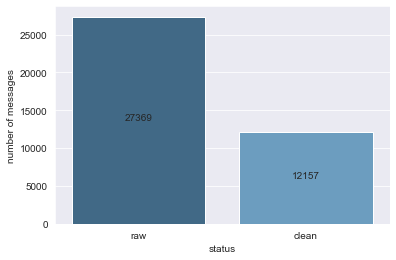
\includegraphics[scale=0.4]{plot-comparison-cleansing-total}
        \caption{Comparison in general}
        \label{fig:plot-comparison-cleansing}
    \end{subfigure}
    \begin{subfigure}{0.5\textwidth}
        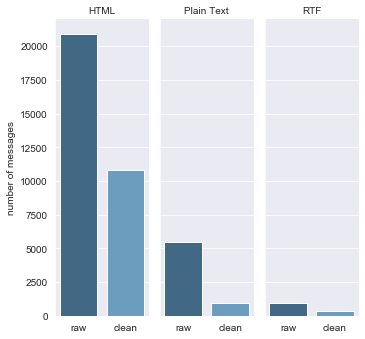
\includegraphics[scale=0.4]{plot-comparison-cleansing-type}
        \caption{Comparison grouped by type}
        \label{fig:plot-comparison-cleansing-types}
    \end{subfigure}
    \caption{Comparison before and after data cleansing}
\end{figure}

\section{Data Labelling}

In supervised learning a model needs to know the correct classification of the samples to compare them against its own predictions. The data set is called pre-labelled. An inevitable part of a data scientist's work is to label data manually. \emph{Doccano}\footnote{available at \url{https://doccano.herokuapp.com}} is an open-source text annotation tool built for creating labelled data. It supports sequence to sequence labelling which is useful for named-entity recognition.

\begin{figure}[!ht]
    \centering
    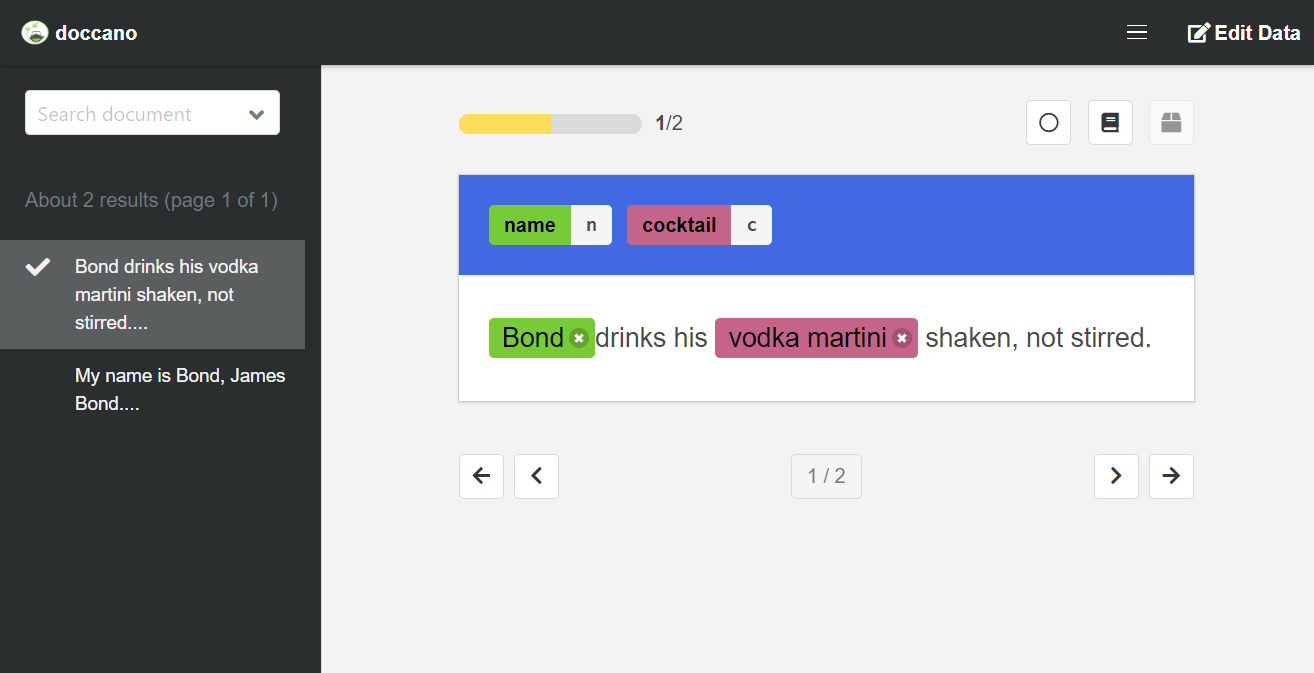
\includegraphics[scale=0.4]{doccano-example}
    \caption{Doccano annotation view}
    \label{fig:doccano-example}
\end{figure}

An advantage of \emph{Doccano} is the graphical user interface which helps you label data manually. You can even define shortcuts to speed up the labelling process.

\subsection{Doccano Parser}

One downside of Doccano are the limited options for exporting labelled data. You can download data only as JSON file with text labels. The exported file has the same structure as listing \ref{code:doccano-export}. If the exported data should be used as validation set it needs to become more handy to work with. Therefore I created a python library called \emph{mobi\_docparser}. The library allows users to parse Doccano's offset notation into a list with two elements: The text after a simple whitespace tokenisation and the corresponding labels for each token, either in IOB or binary notation. After parsing, the named-entity \emph{vodka martini} would be split into the tokens \emph{vodka} (B-DRINK) and \emph{martini} (I-DRINK).

\begin{lstlisting}[label={code:doccano-export}, caption=Sample export from Doccano as JSON (text labels)]
{
  "id": 12162,
  "text": "Bond drinks his vodka martini shaken, not stirred.",
  "meta": {},
  "annotation_approver": null,
  "labels": [[0, 4, "per"], [16, 29, "drink"]]
}
\end{lstlisting}

The offset notation defines named entities by their position inside the text. In the example above, the person entity \emph{Bond} starts at index \emph{0} and ends before index \emph{4}. It's very common in programming, that the second argument doesn't point at the ending token but at the token right after the marked sequence.

\subsection{Annotation Standards}

Named entities need to be described in a standardised way so that ML models can interpret them. There exist a few annotation standards which are often used in NER. If you have to chose a specific labelling standard, keep in mind that sophisticated labelling techniques give you more information than e.g. binary labelling. You can always downgrade to a lower standard but getting distinctive labels out of binary tags isn't possible. On the other hand, it's often easier to label data with low-level tags rather than e.g. IOB tags.

\subsubsection{Binary}

Binary tagging is the simplest form of labelling data. Every token which isn't a named entity is going to be labelled as 0. The remaining tokens which are all entities are tagged with 1. If multiple label types need to be distinguishable, binary tagging isn't the preferred method. As you can see in table \ref{tbl:binary-labelling}, the two entities \emph{people} and \emph{food} cannot be distinguished.

\begin{table}[h!]
    \centering
    \begin{tabular}{|c|c|c|c|c|c|c|c|}
        \hline
        Bond & drinks & his & vodka & martini & shaken, & not & stirred. \\
        \hline
        1 & 0 & 0 & 1 & 1 & 0 & 0 & 0 \\
        \hline
    \end{tabular}
    \caption{Example of a binary tagged sentence}
    \label{tbl:binary-labelling}
\end{table}

This issue can be solved by using multi-class labelling. This technique uses distinctive labels for every entity type as seen in \ref{tbl:multiclass-labelling}.

\begin{table}[h!]
    \centering
    \begin{tabular}{|c|c|c|c|c|c|c|c|}
        \hline
        Bond & drinks & his & vodka & martini & shaken, & not & stirred. \\
        \hline
        1 & 0 & 0 & 2 & 2 & 0 & 0 & 0 \\
        \hline
    \end{tabular}
    \caption{Example of multi-class tagged sentence}
    \label{tbl:multiclass-labelling}
\end{table}

\subsubsection{IOB (Inside-outside-beginning)}

Unlike binary tags, IOB labels allow you to differentiate between multiple label types. \emph{Bond} and \emph{vodka martini} are clearly not in the same entity group (\ref{tbl:iob-labelling}). Additional to the variable types, IOB tagging indicates multi-token entities as such. In the \emph{IOB2} format, the first token of a sequence is always labelled with the prefix \emph{B-} for beginning, the rest with an \emph{I-} for inside \cite{bio95}.

\begin{table}[h!]
    \centering
    \begin{tabular}{|c|c|c|c|c|c|c|c|}
        \hline
        Bond & drinks & his & vodka & martini & shaken, & not & stirred. \\
        \hline
        B-PER & O & O & B-FOOD & I-FOOD & O & O & O \\
        \hline
    \end{tabular}
    \caption{Example of an IOB tagged sentence}
    \label{tbl:iob-labelling}
\end{table}

As shown in table \ref{tbl:iob-labelling2}, the first two tokens are from the same type but still distinguishable. With binary tags you would most likely interpret both tokens as one large named entity consisting of two separate words.

\begin{table}[ht!]
    \centering
    \begin{tabular}{|c|c|c|c|c|c|}
        \hline
        Huey, & Dewey, & and & Louie & are & triplets. \\
        \hline
        B-PER & B-PER & O & B-PER & O & O \\
        \hline
    \end{tabular}
    \caption{Example of distinctive beginning tags}
    \label{tbl:iob-labelling2}
\end{table}

\subsubsection{BIOES}

The IOB format was later extended by an indicator for single and ending tokens. It's called \emph{BIOES} and can be useful if tokens are processed separately from each other so that the model cannot be able to recognise multi-token values by itself. The \emph{s} stands for single tokens whereas the \emph{e} indicates ending tokens \cite{hofer18}.

\begin{table}[h!]
    \centering
    \begin{tabular}{|c|c|c|c|c|c|c|c|}
        \hline
        Bond & drinks & his & vodka & martini & shaken, & not & stirred. \\
        \hline
        S-PER & O & O & B-FOOD & E-FOOD & O & O & O \\
        \hline
    \end{tabular}
    \caption{Example of an BIOES tagged sentence}
    \label{tbl:bioes-labelling}
\end{table}
